\section{Matrix Addition Implementation}

\subsection{Addition: CPU}

We started by implementing addition implementation on the CPU as a baseline for our GPU benchmarks. It uses a single for-loop to iterate over every entry of the input matrices, and stores the result in the result matrix. The implementation can be seen in listing \ref{lst:cpu_addition_short}. For the full implementation, see listing \ref{lst:cpu_addition} in appendix A. 


\begin{lstlisting}[language=C, caption={CPU addition algorithm}, label={lst:cpu_addition_short}]
bool matrix_addition(matrix_t *matrix_a, matrix_t *matrix_b, matrix_t *matrix_c) {
    // Input validations ...
    int rows = matrix_a->rows;
    int columns = matrix_a->columns;

    for (int i = 0; i < rows * columns; i++)
        matrix_c->values[i] = matrix_a->values[i] + matrix_b->values[i];

    return true;
}
\end{lstlisting}

This implementation breaks the abstraction that the \texttt{float *} represents a matrix, since we iterate over it as an array. This is possible, because the addition algorithm adds the elements from $\mathbf{A}$ and $\mathbf{B}$ pairwise. Therefore we can linearly go through the array.

\begin{wrapfigure}{r}{0.5\textwidth}
    \centering
    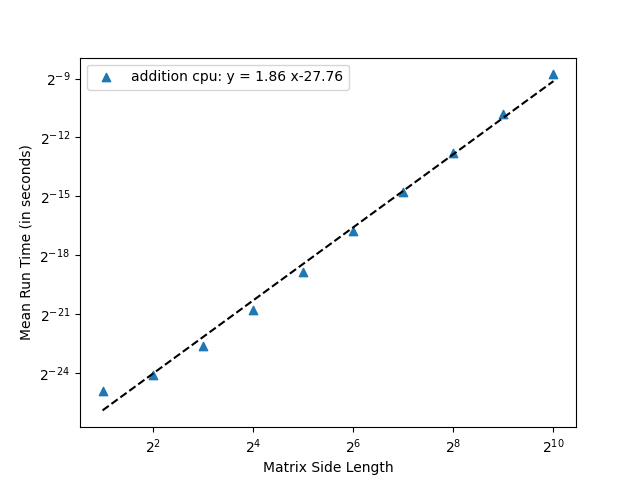
\includegraphics[width=0.5\textwidth]{SavedBenchmarksAndDiagrams/Machine 2/Addition/CPU.png}
    \caption{Addition: CPU Benchmark}
    \label{fig:addition_cpu_bench}
\end{wrapfigure}

Calculating the matrix sum can be done in linear time complexity in the count of matrix elements equal to $O(m * n)$, where $m$ is the row count and $n$ is the column count. For square matrices this can be expressed as $O(n^2)$ for $n^2$ data. 

 For our benchmark diagrams on the CPU, we made a linear regression, that approximates the slope of the algorithm. As can be seen in figure \ref{fig:addition_cpu_bench}, our graph has a slope of $\sim 2$. This is expected, since the algorithm has time complexity $O(n^2)$ and is plotted on logarithmic axes in our diagram (see sect. \ref{subsect:benchmark}). The largest matrix we benchmark has side length 1024. The reason for this will be apparent soon.

Note that for each \texttt{element}, only 1 arithmetic operation has to be performed. The overhead of running this on GPU might outweigh the benefits of parallelization, simply because of the relatively little work each core on the GPU will have to do. Keep this in mind as we dive into the world of GPU programming.

\subsection{Addition: GPU Single Core}
Our first GPU implementation essentially runs our CPU implementation on a single core on the GPU. Again, it runs a single for-loop iterating over every element in the input matrices, adding them, and storing the result in the result matrix (see listing \ref{lst:gpu_addition_single_core}).

\begin{lstlisting}[language=C, caption={GPU addition single core}, label={lst:gpu_addition_single_core}]
__global__ void cuda_matrix_addition_single_core_kernel(
    device_matrix_t matrix_a, device_matrix_t matrix_b,
    device_matrix_t matrix_c, int size, int rows, int columns) {
    for (int i = 0; i < size; i++) {
        matrix_c[i] = matrix_a[i] + matrix_b[i];
    }
}
\end{lstlisting}

For launching kernels we wrote an algorithm runner, which can run any algorithm, which takes three matrices as parameters, as well as three integers. These integers are used for different parameters in our algorithms. For instance in addition, they are the total size of the matrix, the row count and the column count. The total size could be derived from the row and column count, but it is passed as a parameter to precompute it, instead of computing it in each kernel. 

\begin{wrapfigure}{R}{0.5\textwidth}
    \centering
    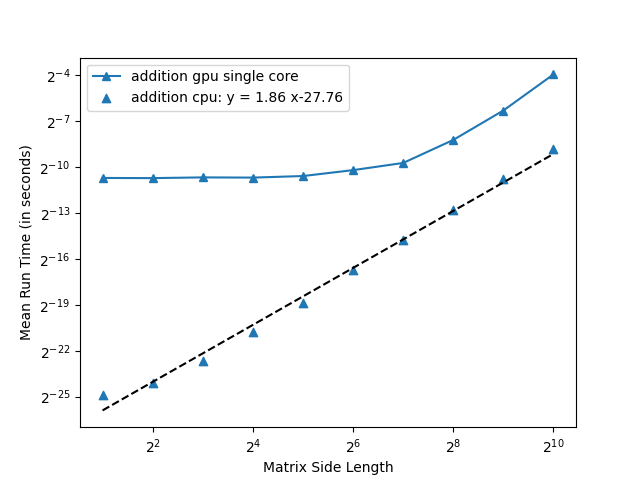
\includegraphics[width=0.5\textwidth]{SavedBenchmarksAndDiagrams/Machine 2/Addition/CPU VS GPU.png}
    \caption{Addition: GPU Single Core Benchmark}
    \label{fig:addition_gpu_sc_bench}
\end{wrapfigure}

We wrote the algorithm runner because much of the code, when writing code for the GPU, is essentially "boilerplate". All addition- and multiplication algorithms requires us to allocate the matrices on the device, copy the matrices over from host to device, run the kernel, and then copy the result matrix back. This "boilerplate" code can be found in listing \ref{lst:algorithm_runner} in appendix A. Launching a kernel requires a grid size and block size. For this implementation both are 1, since we only run code on a single core.

In figure \ref{fig:addition_gpu_sc_bench}, it can be seen that the GPU implementation is a lot slower than the CPU implementation. There might be a few reasons for this. 

The first might be that a single core on the GPU is a lot simpler than the a single core on the CPU, leading to slower performance pr. core, as discussed in \ref{sect:background_gpu}.

Secondly, allocating device memory, copying memory from the host to the device, and launching kernels seems to introduce a lot of overhead. This is apparent on figure \ref{fig:addition_gpu_sc_bench}, since the running time of a matrix of $2^1$ and matrix side length $2^5$ are almost identical. It seems that the increase in work is "drowned out" by the large overhead of running algorithms on the GPU in the first place.

Note that we do not do linear regression for the GPU algorithms, since their diagrams do not exactly follow a linear curve.

\subsection{Addition: GPU Multi Core 1}

\begin{wrapfigure}{R}{0.5\textwidth}
    \centering
    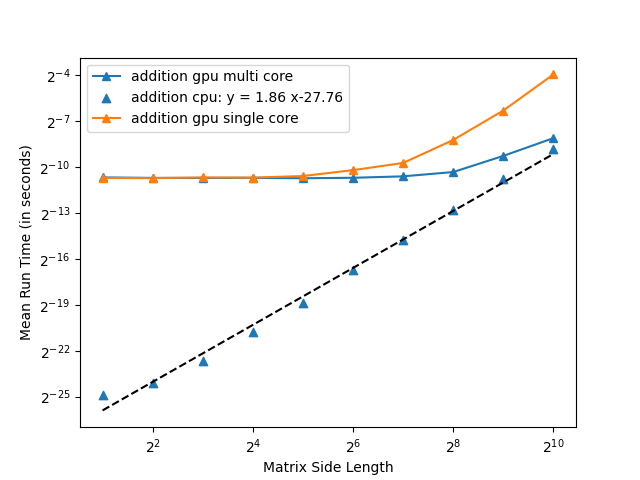
\includegraphics[width=0.5\textwidth]{SavedBenchmarksAndDiagrams/Machine 2/Addition/CPU, GPU SC, GPU MC.png}
    \caption{Addition: GPU Multi Core Benchmark}
    \label{fig:addition_gpu_mc_bench}
\end{wrapfigure}

To get better performance out of the GPU, the following implementation will better utilize its manycore architecture. Instead of calculating all $n$ elements on one core, launch a kernel that has $n$ many threads, utilizing up to $n$ cores at once. Conceptually, the matrix is split up such that each row of the matrix is contained in its own block. Further, each entry of a row is sent to each individual thread of the block. In programming terms, the $i^{th}$ block and the $j^{th}$ thread will be responsible for computing element \texttt{matrix\_c[i][j]} and this element only. 

In listing \ref{lst:gpu_addition_multi_core}, we use the \texttt{blockIdx.x}, \texttt{blockDim.x} and \texttt{threadIdx.x} to calculate which element this thread must work on. These values are available in any kernel, provided by the CUDA library. Note this calculation is essentially the same we used for the \texttt{INDEX} macro, described in section \ref{sect:datastructure}.

\begin{lstlisting}[language=C, caption={GPU addition multi core}, label={lst:gpu_addition_multi_core}]
__global__ void cuda_matrix_addition_multi_core_kernel(
    device_matrix_t matrix_a, device_matrix_t matrix_b, 
    device_matrix_t matrix_c, 
    int size, int rows, int columns) {
    
    int index = blockIdx.x * blockDim.x + threadIdx.x;
    matrix_c[index] = matrix_a[index] + matrix_b[index];
}
\end{lstlisting}

This has one major limitation: NVIDIA allows each block to have at most 1024 threads, so the implementation only works for matrices with a column count of up to 1024. For this reason, the largest matrices we benchmark have side length 1024.

As seen in figure \ref{fig:addition_gpu_mc_bench} the multi core implementation of addition on the GPU is significantly faster than the single core implementation, when the matrices are big enough. While starting at the same point (due to the overhead of utilizing the GPU in the first place), the multi core implementation stays constant for a longer time, before it starts to increase. Its slope is also gentler than the slope of the single core and the CPU implementation.

This is due to the fact that we are now efficiently utilizing the SMs of our GPU. The rise of the slope is due to the fact that we run out of SMs, and the blocks have to wait until an SM is available.

Our implementation is, however, not faster than our CPU implementation. We suspect this is due to the relatively little amount of work this algorithm has for each element. Later in this section we will try to tune the GPU implementation to remedy this.

\subsection{Addition: GPU Multi Core 2}

\begin{wrapfigure}{R}{0.5\textwidth}
    \centering
    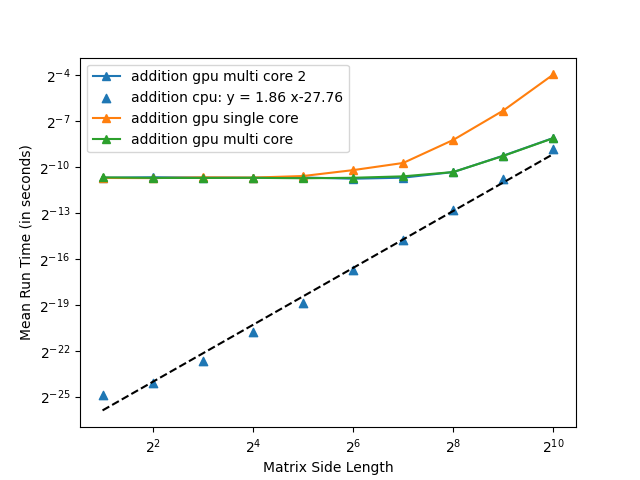
\includegraphics[width=0.5\textwidth]{SavedBenchmarksAndDiagrams/Machine 2/Addition/CPU, GPU SC, GPU MC 1, GPU MC 2.png}
    \caption{Addition: GPU Multi Core 2 Benchmark}
    \label{fig:addition_gpu_mc_2_bench}
\end{wrapfigure}

With this implementation, we will hardcode the number of threads in each block to be 16 x 16. This way, we hope to better take advantage of each multiprocessor and solve the major limitation of the previous algorithm.

Because each SM is responsible for scheduling the execution of blocks, it would not make sense for each block to have 1024 threads that all have to finish before the multiprocessor can schedule a new block. Also, as discussed in \ref{sect:background_gpu}, small blocks allow our algorithm to scale better on a plethora of devices with different SM counts.

Each block will consist of 16 by 16 threads, meaning 256 threads in total. Each grid will consist of $rows / 16$ by $columns / 16$ blocks. To allow for arbitrarily sized matrices, we also included some padding, so the actual grid size is $(rows + 15) / 16$ by $(columns + 15) / 16$. Because of the padding we also need to have a check, so we do not write out of bounds of the array. The implementation can be seen in listing \ref{lst:gpu_addition_multi_core_2}.

\begin{lstlisting}[language=C, caption={GPU addition multi core 2}, label={lst:gpu_addition_multi_core_2}]
__global__ void cuda_matrix_addition_multi_core_kernel2(
    device_matrix_t matrix_a, device_matrix_t matrix_b,
    device_matrix_t matrix_c, 
    int size, int rows, int columns) {
    
    int i = blockIdx.x * blockDim.x + threadIdx.x;
    int j = blockIdx.y * blockDim.y + threadIdx.y;
    if (i >= rows || j >= columns) return;

    matrix_c[INDEX(i, j, columns)] =
        matrix_a[INDEX(i, j, columns)] 
            + matrix_b[INDEX(i, j, columns)];
}
\end{lstlisting}

In figure \ref{fig:addition_gpu_mc_2_bench}, it can be seen that there is no performance increase between this implementation and the previous implementation. We suspect this is because each thread has so little work to do, that it does not matter if the blocks have size 256 or 1024. 

Other than fixing our previous limitation of only allowing matrices of up to side length of 1024, this implementation gives no performance benefits.

\subsection{Addition: GPU Multi Core - Larger Kernels}

\subsection{A note about the choice of data structure}

As mentioned earlier, at the beginning of this project we used a 2D data structure. We implemented CPU addition, GPU single core addition and the first GPU multi core addition. On the GPU side it was still simply a \texttt{float *}, and we would simply flatten the two-dimensional matrix to a 1-dimensional one and send it over to the GPU. When we got the result matrix back from the GPU we would turn it back into a two-dimensional data structure. 

We suspected that this translation between the two representations might have introduced some overhead. Therefore we decided to pivot to a fully one-dimensional approach. We decided to benchmark the two data structures against each other for both the CPU and GPU. As can be seen in figure \ref{fig:1d_vs_2d_bench}, all of the algorithms run faster with the one-dimensional approach, rather than the two-dimensional one, even on the CPU. This is likely due to the fact that our CPU implementation of addition iterates over the matrix linearly, giving optimal locality in the one-dimensional approach.

\begin{figure}[ht]
    \centering
    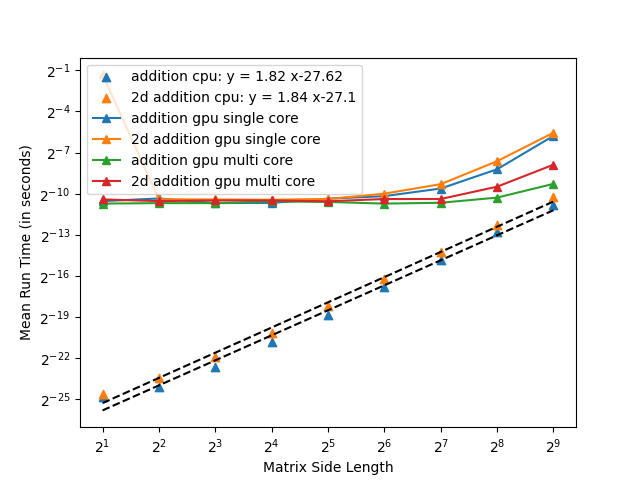
\includegraphics[width=0.65\textwidth]{SavedBenchmarksAndDiagrams/Machine 2/2D vs 1D.png}
    \caption{CPU Addition Benchmark}
    \label{fig:1d_vs_2d_bench}
\end{figure}
